% Provenance (never printed): see sources/outline_sources.md (Year 3:
% ocean dynamics: the Ekman layer derived, the Sverdrup balance, western
% intensification, the abyssal circulation, ocean tides).
% Brief: sources/book5/BRIEFS.md, ch. 21. Curves from
% figdata/bachelor-3/wind_driven_gyre.py and tides.py. Exercise and problem
% values in the Book 5 scratch calculator calc/ch21.py. The basins, winds
% and stations of the exercises and the problem are invented.
\chapter{Dinámica oceánica}\label{ch:b3:ocean-dynamics}

A través del estrecho de Florida, la corriente del Golfo transporta unos
\qty{32}{\sverdrup} de agua hacia el norte, y crece a medida que sigue la costa
hacia el norte, hasta unos \qty{150}{\sverdrup} cerca de \ang{40} N. Al otro lado del mismo océano, frente a Portugal y el norte
de África, nada parecido fluye hacia el sur: el agua que transporta la corriente del Golfo
al norte regresa hacia el ecuador como una deriva lenta y amplia a lo largo de miles
de kilómetros de mar abierto. Todas las cuencas oceánicas del hemisferio norte presentan
la misma forma asimétrica, con su corriente rápida en el lado occidental. La
asimetría se debe al viento, a la fricción del mar y a un
hecho relativo a la Tierra: el parámetro de Coriolis crece hacia el polo.
% ledger: rapid:transports (31.7 Sv, rounded), stewart:north-atlantic

\begin{recall}
La fuerza de marea de la Luna y del Sol, las mareas vivas y muertas, se estudian en los
libros de física. La tensión del viento, la capa de Ekman, el transporte de Ekman y
la espiral de Ekman, el afloramiento y el hundimiento, los giros, las corrientes
de frontera occidental, el sverdrup ($\qty{1}{\sverdrup} =
\qty{e6}{m^3/s}$), la circulación meridional de vuelco y la
formación de aguas profundas están en el volumen de primer año, en su capítulo sobre la
circulación oceánica; allí la tensión del viento se escribe $\vec T$, aquí
$\vec\tau$. El parámetro de Coriolis, el plano $\beta$, el radio de Rossby
y el equilibrio geostrófico se encuentran en el capítulo~\ref{ch:b3:gfd-foundations};
la vorticidad y la \omterm{def:b3:atmospheric-dynamics:pv}{vorticidad potencial}, en el capítulo~\ref{ch:b3:atmospheric-dynamics}.
\end{recall}

\section{La capa de Ekman deducida}\label{sec:b3:ocean-dynamics:ekman}

En el volumen de primer año el transporte de Ekman se obtuvo a partir de un balance de fuerzas
sobre toda la capa, y la espiral de velocidades en su interior se enunció. Con
una fricción turbulenta de viscosidad de remolino constante $A_z$, la espiral se deduce
de las ecuaciones en unas pocas líneas. Se escribe la velocidad horizontal como un
número complejo, $W = u + \mathrm iv$, y la tensión del viento como $\tau =
\tau_x + \mathrm i\tau_y$; una multiplicación por $-\mathrm i$ gira un vector
\ang{90} en sentido horario, hacia su derecha vista desde arriba.

\begin{theorem}[Perfil de velocidades de una capa superficial estacionaria impulsada por el viento]\label{thm:b3:ocean-dynamics:ekman}
En un océano estacionario, horizontalmente uniforme, de gran profundidad y densidad constante
$\rho$, con una viscosidad de remolino vertical constante $A_z$ y el parámetro de Coriolis
$f > 0$, la corriente impulsada por una tensión del viento $\tau$ es
\[
W(z) = W_0\,\mathrm e^{(1+\mathrm i)z/\delta},\qquad
W_0 = \frac{\tau}{\rho\sqrt{fA_z}}\,\mathrm e^{-\mathrm i\pi/4},\qquad
\delta = \sqrt{\frac{2A_z}{f}} ,
\]
para $z \le 0$. La corriente superficial gira \ang{45} a la derecha de la
tensión; con la profundidad gira aún más a la derecha y decae como $\mathrm
e^{z/\delta}$; el transporte total $\int_{-\infty}^0 W\,\mathrm dz =
-\mathrm i\tau/(\rho f)$ es perpendicular a la tensión y queda a su derecha.
\end{theorem}

\begin{proof}
Lejos de las costas no hay gradiente horizontal de presión en la capa,
y la fuerza de Coriolis equilibra la fricción: $-fv = A_z u''$ y $fu =
A_z v''$, siendo los apóstrofos derivadas en $z$. Multiplicando la segunda por
$\mathrm i$ y sumando se obtiene $A_zW'' = \mathrm ifW$. Sus soluciones son
$\mathrm e^{\pm(1+\mathrm i)z/\delta}$, ya que $(1+\mathrm i)^2/\delta^2 =
2\mathrm i/\delta^2 = \mathrm if/A_z$; solo el signo más permanece acotado cuando
$z \to -\infty$. En la superficie la tensión la transmite la fricción,
$\rho A_zW'(0) = \tau$, luego $W_0 = \tau\delta/(\rho A_z(1+\mathrm i))$.
Como $\delta/(\sqrt2 A_z) = 1/\sqrt{fA_z}$ y $1/(1+\mathrm i) = \mathrm
e^{-\mathrm i\pi/4}/\sqrt2$, esto es el $W_0$ enunciado. El factor
$\mathrm e^{\mathrm iz/\delta}$ gira en sentido horario al disminuir $z$. Por último
$\int_{-\infty}^0 W\,\mathrm dz = W_0\delta/(1+\mathrm i) =
\tau\delta^2/(\rho A_z(1+\mathrm i)^2) = \tau\delta^2/(2\mathrm i\rho A_z)
= -\mathrm i\tau/(\rho f)$.
\end{proof}

El teorema recupera los dos resultados del volumen de primer año: la corriente superficial de Ekman
a \ang{45} y el transporte $\tau/(\rho f)$, perpendicular a
la tensión e independiente de $A_z$, que nunca se conoce bien. A la
profundidad $\pi\delta$ la corriente fluye en sentido contrario a la superficial, reducida
por $\mathrm e^{-\pi}$, hasta \qty{4}{\percent}.

\begin{definition}[Profundidad de Ekman; bombeo de Ekman]\label{def:b3:ocean-dynamics:ekman-pumping}
La \emph{profundidad de Ekman}\index{profundidad de Ekman} es $D_E = \pi\delta =
\pi\sqrt{2A_z/f}$, la profundidad a la que la corriente de la espiral de Ekman
fluye en sentido opuesto a la corriente superficial; mide el espesor de la
capa de Ekman. El \emph{bombeo de Ekman}\index{bombeo de Ekman} es la
velocidad vertical $w_E$ en la base de la capa de Ekman, forzada por la convergencia o
divergencia del transporte de Ekman: hacia abajo donde los transportes
convergen, hacia arriba, llamada a veces succión de Ekman, donde divergen.
\end{definition}

\begin{proposition}[Bombeo de Ekman]\label{prop:b3:ocean-dynamics:pumping}
Con la velocidad vertical nula en la superficie del mar, el \omterm{def:b3:ocean-dynamics:ekman-pumping}{bombeo de Ekman} es
\[
w_E = \operatorname{curl}_z\frac{\vec\tau}{\rho f}
= \frac{1}{\rho f}\Big(\frac{\partial\tau_y}{\partial x} -
\frac{\partial\tau_x}{\partial y}\Big) + \frac{\beta\tau_x}{\rho f^2} ,
\]
con signo positivo hacia arriba.
\end{proposition}

\begin{proof}
El transporte de volumen de la capa es $(U_E, V_E) = (\tau_y,
-\tau_x)/(\rho f)$, el teorema escrito en componentes. Integrando la
ecuación de continuidad $\partial w/\partial z = -(\partial u/\partial x +
\partial v/\partial y)$ a través de la capa, $w(0) - w_E = -(\partial
U_E/\partial x + \partial V_E/\partial y)$, luego $w_E = \partial_x(\tau_y/\rho
f) - \partial_y(\tau_x/\rho f)$. Desarrollando con $\mathrm df/\mathrm dy =
\beta$ se obtiene la segunda forma.
\end{proof}

Un viento que gira ciclónicamente sobre el mar, con rotacional positivo, hace subir
agua desde debajo de la capa; un viento anticiclónico la empuja hacia abajo. Sobre
los océanos subtropicales, los alisios soplan del este en el
lado ecuatorial, y los vientos del oeste por el lado polar. Sus transportes de Ekman
se dirigen hacia el norte bajo los alisios y hacia el sur bajo los vientos del oeste,
convergen entre ellos: el agua superficial se acumula y se bombea hacia abajo, como
muestra la figura siguiente. A lo largo de una costa donde el
viento sopla con la costa a su izquierda (en el hemisferio norte), el
transporte se aleja de la orilla y el afloramiento costero del volumen de primer año
es una succión de Ekman concentrada contra una pared.

\begin{omfigure}
\centering
\begin{tikzpicture}[>=stealth, font=\small, x=1.1cm, y=1cm]
\fill[omThm!7] (-5,0) rectangle (5,-3.6);
\draw[thick] (-5,0) -- (5,0);
\draw[black!45, densely dashed] (-5,-0.9) -- (5,-0.9);
\node[font=\scriptsize, black!60, anchor=north east, inner sep=1pt] at (4.95,-0.95) {capa de Ekman};
% winds: west is out of the page, east into the page
\foreach \x in {-4.2,-3.4,-2.6} {\draw (\x,0.55) circle (0.13); \fill (\x,0.55) circle (0.04);}
\foreach \x in {2.6,3.4,4.2} {\draw (\x,0.55) circle (0.13);
  \draw (\x-0.09,0.46) -- (\x+0.09,0.64); \draw (\x-0.09,0.64) -- (\x+0.09,0.46);}
\node[above] at (-3.4,0.75) {alisios, desde el este};
\node[above] at (3.4,0.75) {vientos del oeste, desde el oeste};
% Ekman transports converge
\draw[->, omDef, very thick] (-4.5,-0.45) -- (-1.2,-0.45);
\draw[->, omDef, very thick] (4.5,-0.45) -- (1.2,-0.45);
\node[omDef, font=\scriptsize, fill=omThm!7, inner sep=1pt] at (-2.85,-0.72) {transporte de Ekman};
% pumping
\foreach \x in {-0.6,0,0.6} \draw[->, omThm, thick] (\x,-0.55) -- (\x,-1.55);
\node[omThm, font=\scriptsize, anchor=west] at (0.75,-1.25) {$w_E < 0$};
% squashed column and Sverdrup flow
\draw[thick, black!70] (-0.62,-1.75) rectangle (0.62,-3.1);
\node[font=\scriptsize, black!70, align=center] at (0,-2.42) {columna\\comprimida};
\draw[->, omMeth, very thick] (-0.75,-2.42) -- (-3.2,-2.42);
\node[omMeth, font=\scriptsize, align=center, above] at (-2.6,-2.40) {flujo de Sverdrup,\\hacia el ecuador};
\draw[black!45, densely dashed] (-5,-3.3) -- (5,-3.3);
\node[font=\scriptsize, black!60, anchor=south east, inner sep=1pt] at (4.95,-3.28) {base del flujo impulsado por el viento};
\node[below, font=\scriptsize] at (-5,-3.6) {sur};
\node[below, font=\scriptsize] at (5,-3.6) {norte};
\end{tikzpicture}

\par\smallskip{\small Sección norte--sur a través de un giro subtropical
del hemisferio norte, con el este hacia el interior de la página. Los transportes de Ekman bajo
los alisios y los vientos del oeste convergen, el agua se bombea hacia abajo, y las
columnas inferiores, aplastadas, se desplazan hacia el ecuador, donde $f$ es menor,
para conservar su \omterm{def:b3:atmospheric-dynamics:pv}{vorticidad potencial}.}\label{fig:b3:ocean-dynamics:pumping}
\end{omfigure}

\section{El equilibrio de Sverdrup}\label{sec:b3:ocean-dynamics:sverdrup}

Por debajo de la capa de Ekman el océano es geostrófico. Una columna de agua que es
aplastada por el \omterm{def:b3:ocean-dynamics:ekman-pumping}{bombeo de Ekman} debe, para conservar su \omterm{def:b3:atmospheric-dynamics:pv}{vorticidad potencial} $f/h$,
desplazarse hacia donde $f$ es menor: hacia el ecuador. En 1947 H.~U.~Sverdrup
cuantificó el argumento para toda la profundidad del flujo impulsado por el viento.
% ledger: stewart:ekman-layer (Sverdrup 1947)

\begin{theorem}[Equilibrio de Sverdrup]\label{thm:b3:ocean-dynamics:sverdrup}
En un océano estacionario en el que los términos no lineales y la fricción lateral
son despreciables, el interior es geostrófico por debajo de la capa de Ekman, y la
velocidad vertical se anula a cierta profundidad $-H$, el transporte total de volumen hacia el norte
por unidad de anchura del flujo impulsado por el viento obedece al \emph{equilibrio
de Sverdrup}\index{equilibrio de Sverdrup}
\[
\beta V = \frac{1}{\rho}\operatorname{curl}_z\vec\tau
= \frac{1}{\rho}\Big(\frac{\partial\tau_y}{\partial x} -
\frac{\partial\tau_x}{\partial y}\Big) .
\]
\end{theorem}

\begin{proof}
En el interior geostrófico $fv_g = \rho^{-1}\partial p/\partial x$ y
$fu_g = -\rho^{-1}\partial p/\partial y$. Por tanto $\partial_x(fu_g) +
\partial_y(fv_g) = 0$, es decir, $f(\partial_xu_g + \partial_yv_g) + \beta
v_g = 0$, y con la continuidad, $\beta v_g = f\,\partial w/\partial z$.
Integrando desde $-H$, donde $w = 0$, hasta la base de la capa de Ekman,
donde $w = w_E$, se obtiene $\beta V_g = fw_E$. Por
la \cref{prop:b3:ocean-dynamics:pumping}, $fw_E = \rho^{-1}\operatorname{curl}_z
\vec\tau + \beta\tau_x/(\rho f)$. Sumando el transporte de Ekman $V_E =
-\tau_x/(\rho f)$, multiplicado por $\beta$, cancela el último término:
$\beta(V_g + V_E) = \rho^{-1}\operatorname{curl}_z\vec\tau$.
\end{proof}

El equilibrio es notable por lo que no necesita: ni la profundidad del
flujo, ni su estructura vertical, ni la viscosidad de remolino, solo el
rotacional del viento y $\beta$. Sverdrup lo dedujo de las ecuaciones de
movimiento integradas hasta una profundidad de no movimiento, y lo contrastó con las
secciones hidrográficas de los buques de investigación \emph{Carnegie} y
\emph{Bushnell} en el Pacífico tropical oriental, entre \ang{34} N y
\ang{10} S, con una profundidad de no movimiento de \qty{1000}{m}: los transportes
calculados a partir del viento coincidían con los calculados a partir del campo de densidad, incluso
donde las corrientes iban en contra del viento. Trabajos posteriores con vientos de mejor calidad
hallaron el mejor acuerdo con una profundidad de no movimiento cercana a \qty{500}{m}, y
las medidas del esfuerzo medio en el Pacífico ecuatorial en 1999 hallaron que el
flujo allí se hallaba en \omterm{thm:b3:ocean-dynamics:sverdrup}{equilibrio de Sverdrup}. Si el equilibrio se cumple en todas partes es
más difícil de demostrar que de suponer: casi toda teoría de la circulación oceánica
parte de él.
% ledger: stewart:sverdrup

Considérese la cuenca ficticia del problema de este capítulo: entre \ang{20} y
\ang{50} N, de \qty{6000}{km} de anchura, bajo un esfuerzo zonal $\tau_x =
-\tau_0\cos(\pi(\varphi - \ang{20})/\ang{30})$ con $\tau_0 =
\qty{0.1}{Pa}$, de componente este en \ang{20} N, de componente oeste en \ang{50} N, nulo en
\ang{35} N. En casi toda la cuenca el rotacional del esfuerzo es negativo: el
agua se bombea hacia abajo, unos \qty{35}{m} al año a \ang{35} N, y el
interior fluye hacia el sur, \qty{4.9}{m^2/s} por metro de anchura a \ang{35} N,
\qty{29.4}{\sverdrup} a través de la cuenca. Calculado a partir de los vientos observados,
el transporte de Sverdrup del giro subtropical del Atlántico Norte alcanza unos
\qty{30}{\sverdrup} cerca de \ang{28} N.
% ledger: stewart:north-atlantic (computed in figdata/bachelor-3/wind_driven_gyre.py)

\begin{omfigure}
\begin{tikzpicture}
\begin{groupplot}[group style={group size=3 by 1, horizontal sep=0.45cm, yticklabels at=edge left},
  width=0.37\linewidth, height=0.46\linewidth, ymin=20, ymax=50, ytick={20,25,30,35,40,45,50},
  tick label style={font=\scriptsize}, label style={font=\small}, title style={font=\small}]
\nextgroupplot[xlabel={$\tau_x$ (\unit{Pa})}, ylabel={latitud (\unit{\degree} N)},
  xmin=-0.12, xmax=0.12, xtick={-0.1,0,0.1}, title={tensión del viento},
  scaled x ticks=false, xticklabel style={/pgf/number format/fixed}]
% computed in figdata/bachelor-3/wind_driven_gyre.py
\addplot[black!50, thin] coordinates {(0,20) (0,50)};
\addplot[omThm, thick] table[x=tau, y=lat] {figdata/out/bachelor-3-wind_driven_gyre-merid.dat};
\nextgroupplot[xlabel={$w_E$ (\unit{m/yr})}, xmin=-45, xmax=12, xtick={-40,-20,0},
  title={bombeo de Ekman}]
\addplot[black!50, thin] coordinates {(0,20) (0,50)};
\addplot[omDef, thick] table[x=wE, y=lat] {figdata/out/bachelor-3-wind_driven_gyre-merid.dat};
\nextgroupplot[xlabel={transporte (\unit{\sverdrup})}, xmin=-32, xmax=10, xtick={-30,-20,-10,0,10},
  title={Sverdrup}]
\addplot[black!50, thin] coordinates {(0,20) (0,50)};
\addplot[omMeth, thick] table[x=Vtot, y=lat] {figdata/out/bachelor-3-wind_driven_gyre-merid.dat};
\end{groupplot}
\end{tikzpicture}

\par\smallskip{\small La cuenca ficticia del problema, \ang{20} a
\ang{50} N y \qty{6000}{km} de anchura. A la izquierda, la tensión zonal del viento, con sentido
positivo hacia el este. En el centro, el \omterm{def:b3:ocean-dynamics:ekman-pumping}{bombeo de Ekman}, con signo positivo hacia arriba: el agua se empuja
hacia abajo al sur de \ang{47} N, con más intensidad en el sur, donde $f$ es pequeño,
y se eleva al norte de esa latitud. A la derecha, el transporte de Sverdrup total hacia el norte a través de la cuenca:
el interior va hacia el sur, \qty{29.4}{\sverdrup} a \ang{35} N, salvo en una
franja delgada en el borde norte, donde el rotacional del esfuerzo cambia de signo.}\label{fig:b3:ocean-dynamics:sverdrup}
\end{omfigure}
% ledger: earth:Rmean, geod5:grs80-defining

El transporte de Sverdrup fija $V$ en cada punto, pero una función de corriente
necesita una condición de contorno, y una pared meridional solo admite una. Si el
interior satisface la condición de no flujo a través de la pared oriental, el flujo hacia el sur
no tiene por dónde salir en la pared occidental; la masa es devuelta por una corriente
que las ecuaciones de Sverdrup, sin fricción, no pueden describir.

\section{Intensificación occidental}\label{sec:b3:ocean-dynamics:western}

En 1948 H.~Stommel añadió la fricción más sencilla al océano más sencillo, y
halló el flujo de retorno concentrado contra la pared occidental, como en la
figura del volumen de primer año sobre su giro. Lo halló solo con un
parámetro de Coriolis que crece hacia el norte: sin rotación, o con uno uniforme,
su giro era simétrico.
% ledger: stewart:stommel, stommel:1948

\begin{definition}[Intensificación occidental; modelo de Stommel; capa límite de Munk]\label{def:b3:ocean-dynamics:western-intensification}
La \emph{intensificación occidental}\index{intensificación occidental} es la
concentración del flujo de retorno de un giro impulsado por el viento en una corriente
estrecha y rápida junto al lado occidental de la cuenca. El \emph{modelo de
Stommel}\index{modelo de Stommel} es un océano homogéneo de profundidad constante en una
cuenca rectangular, impulsado por una tensión zonal del viento y frenado por una
fricción de fondo proporcional a la velocidad integrada en la profundidad, con un coeficiente $r$;
su función de corriente de transporte $\psi$ ($U = -\partial\psi/\partial y$, $V =
\partial\psi/\partial x$) obedece
\[
r\nabla^2\psi + \beta\frac{\partial\psi}{\partial x} =
\frac{1}{\rho}\operatorname{curl}_z\vec\tau ,\qquad \psi = 0 \text{ en las paredes.}
\]
La \emph{capa límite de Munk}\index{capa límite de Munk} es la
capa límite occidental del mismo giro cuando una viscosidad de remolino lateral $A_H$
sustituye a la fricción de fondo; su escala de anchura es $\delta_M =
(A_H/\beta)^{1/3}$.
\end{definition}

La ecuación es el \omterm{thm:b3:ocean-dynamics:sverdrup}{equilibrio de Sverdrup} con el rotacional de la fricción de fondo
añadido: integrada en la profundidad, $\beta V = \rho^{-1}\operatorname{curl}_z
\vec\tau - r\zeta_T$, donde $\zeta_T = \nabla^2\psi$ es la vorticidad del
transporte.

\begin{theorem}[Capa límite occidental del giro de Stommel]\label{thm:b3:ocean-dynamics:stommel}
En una cuenca $0 \le x \le X$, $0 \le y \le L$, con $\tau_x = -\tau_0
\cos(\pi y/L)$ y $\delta_S = r/\beta \ll X$, la función de corriente de Stommel
es, a primer orden en $\delta_S/X$,
\[
\psi = A\sin\frac{\pi y}{L}\Big[(X - x) - X\mathrm e^{-x/\delta_S}\Big],
\qquad A = \frac{\pi\tau_0}{\rho\beta L} .
\]
El interior transporta $AX\sin(\pi y/L)$ hacia el sur; una capa límite de anchura
$\delta_S$ junto a la pared occidental lo devuelve hacia el norte; no puede haber capa límite
que exista junto a la pared oriental.
\end{theorem}

\begin{proof}
El rotacional del esfuerzo es $-\partial\tau_x/\partial y = -(\pi\tau_0/L)\sin(\pi
y/L)$. A lo ancho de la cuenca el término de fricción es menor que el
término $\beta$ en una proporción $\delta_S/X$; al despreciarlo queda el \omterm{thm:b3:ocean-dynamics:sverdrup}{equilibrio de Sverdrup},
$\beta\,\partial\psi/\partial x = -(\pi\tau_0/\rho L)\sin(\pi y/L)$, cuya
solución que se anula en $x = X$ es $\psi_I = A\sin(\pi y/L)(X - x)$. Esta
no se anula en $x = 0$. Cerca de una pared $\psi$ varía rápidamente en $x$, y la
ecuación se reduce a $r\,\partial^2\psi/\partial x^2 + \beta\,\partial\psi/
\partial x = 0$ para la corrección, cuyas soluciones son una constante y
$\mathrm e^{-x/\delta_S}$. Esta última decae hacia el este, alejándose de la
pared occidental: al añadir $-AX\sin(\pi y/L)\,\mathrm e^{-x/\delta_S}$ se hace $\psi = 0$
en $x = 0$ y no cambia nada en el interior. En la pared oriental una
corrección tendría que decaer hacia el oeste, alejándose de $x = X$, y
$\mathrm e^{-x/\delta_S}$ crece hacia el oeste: no existe tal capa, así que el
interior debe encontrar la pared oriental por sí solo, como lo hace $\psi_I$. La
transporte hacia el norte entre la pared y el punto donde $V$ cambia de signo
es allí $\psi$, próximo a $AX\sin(\pi y/L)$.
\end{proof}

La misma respuesta se obtiene a partir de la vorticidad. En el interior, el viento proporciona
a cada columna vorticidad negativa, y la columna lo compensa desplazándose
hacia el sur, hacia valores menores de $f$. Al volver al norte gana \omterm{def:b3:atmospheric-dynamics:vorticity-kinds}{vorticidad planetaria}
y debe perderla, algo que solo puede hacer la fricción. En una corriente hacia el norte
cuya velocidad disminuye hacia el este desde las cercanías de la pared occidental, $\partial
v/\partial x < 0$ en la mayor parte de su anchura: la vorticidad de la corriente es negativa, y la fricción, que actúa en contra
de ella, aporta la vorticidad positiva que necesitan las columnas. Una corriente hacia el norte
junto a una pared oriental tendría vorticidad positiva, y
la fricción quitaría el signo equivocado.

\begin{omfigure}
\begin{tikzpicture}
\begin{groupplot}[group style={group size=2 by 1, horizontal sep=1.7cm},
  width=0.48\linewidth, height=0.42\linewidth, xmin=0, xmax=400,
  xlabel={distancia a la pared occidental (\unit{km})},
  tick label style={font=\scriptsize}, label style={font=\small},
  legend style={font=\scriptsize, draw=none, fill=none}]
\nextgroupplot[ylabel={$V$ (\unit{m^2/s})}, ymin=-80, ymax=600, legend pos=north east,
  legend cell align=left]
% computed in figdata/bachelor-3/wind_driven_gyre.py
\addplot[omThm, thick] table[x=x, y=vS] {figdata/out/bachelor-3-wind_driven_gyre-bl.dat};
\addlegendentry{Stommel, $\delta_S = \qty{53}{km}$}
\addplot[omDef, thick] table[x=x, y=vM] {figdata/out/bachelor-3-wind_driven_gyre-bl.dat};
\addlegendentry{Munk, $\delta_M = \qty{64}{km}$}
\addplot[black!50, thin, forget plot] coordinates {(0,0) (400,0)};
\nextgroupplot[ylabel={transporte desde la pared (\unit{\sverdrup})}, ymin=0, ymax=36,
  legend pos=south east, legend cell align=left]
\addplot[omThm, thick] table[x=x, y=cS] {figdata/out/bachelor-3-wind_driven_gyre-bl.dat};
\addlegendentry{Stommel}
\addplot[omDef, thick] table[x=x, y=cM] {figdata/out/bachelor-3-wind_driven_gyre-bl.dat};
\addlegendentry{Munk}
\addplot[black!60, densely dashed] coordinates {(0,29.4) (400,29.4)};
\addlegendentry{interior, \qty{29.4}{\sverdrup}}
\end{groupplot}
\end{tikzpicture}

\par\smallskip{\small La capa límite occidental en el centro de la
cuenca ficticia del problema (\ang{35} N, \qty{6000}{km} de anchura). A la izquierda, el
transporte hacia el norte por unidad de anchura: la capa de Stommel, con una fricción de fondo
$r = \qty{e-6}{s^{-1}}$, decae exponencialmente desde la pared; la de Munk, con
$A_H = \qty{5e3}{m^2/s}$ y sin deslizamiento en la pared, crece desde cero y alcanza un máximo
a unos \qty{80}{km} de distancia y va seguido de una débil contracorriente hacia el sur.
A la derecha, el transporte entre la pared y cada distancia, frente al
\qty{29.4}{\sverdrup} que el interior transporta hacia el sur: la capa de Stommel
acumula \qty{27.9}{\sverdrup} antes de que su flujo gire hacia el sur, y el chorro de Munk
\qty{33.0}{\sverdrup} antes de su contracorriente.}\label{fig:b3:ocean-dynamics:boundary}
\end{omfigure}
% ledger: stewart:munk

Con $r = \qty{e-6}{s^{-1}}$ a \ang{35} N, $\delta_S = \qty{53}{km}$, y
el flujo hacia el norte ocupa los primeros \qty{250}{km} desde la pared. En 1950
W.~H.~Munk sustituyó la fricción de fondo por una viscosidad lateral de remolino $A_H$,
que actúa sobre la cizalla dentro de la corriente; la ecuación gana un término
$A_H\nabla^4\psi$, y cerca de la pared occidental la corrección se convierte en
$\mathrm e^{-x/2\delta_M}$ multiplicada por una oscilación, $\cos(\sqrt3x/2\delta_M)$
y $\sin(\sqrt3x/2\delta_M)$. Con $A_H = \qty{5e3}{m^2/s}$ el chorro hacia el norte
tiene unos \qty{225}{km} de anchura (\qty{233}{km} en la cuenca de la figura),
con una débil contracorriente más allá, una forma semejante a la de la corriente del Golfo y
la corriente de Kuroshio. Como en la capa de Stommel, el transporte del chorro no
depende de la fricción, sino solo del rotacional de la tensión del viento, de la anchura de la
cuenca y de $\beta$. Con los vientos de su época, Munk calculó
\qty{36}{\sverdrup} para la corriente del Golfo y \qty{39}{\sverdrup} para la
corriente de Kuroshio, aproximadamente la mitad de los transportes medidos entonces; con un mejor
coeficiente de arrastre y promedios más finos de la tensión del viento, se obtuvo \qty{32}{\sverdrup}
para la corriente del Golfo en 1978. Medida sobre todo con un cable submarino, la
corriente del Golfo en el estrecho de Florida ha transportado \qty{31.7}{\sverdrup} de
media desde 2004. Aguas abajo crece hasta unos \qty{150}{\sverdrup} cerca de
\ang{40} N, y mar adentro del cabo Hatteras una fuerte recirculación, que la
teoría lineal no contiene, deteriora el acuerdo.
% ledger: stewart:munk, rapid:transports, stewart:north-atlantic

\section{La circulación abisal}\label{sec:b3:ocean-dynamics:abyssal}

El océano profundo se alimenta desde unos pocos lugares. En el volumen de primer año, el agua profunda
se forma donde el agua superficial se enfría y se vuelve densa en el lejano Atlántico Norte
y alrededor de la Antártida, y se extiende por las cuencas como
agua profunda del Atlántico Norte y agua de fondo antártica. Entre 1958 y 1960
H.~Stommel, A.~B.~Arons y A.~J.~Faller preguntaron cómo se extiende, empleando el
mismo argumento de vorticidad que Sverdrup.

\begin{definition}[Modelo de Stommel--Arons]\label{def:b3:ocean-dynamics:abyssal}
El \emph{modelo de Stommel--Arons}\index{modelo de Stommel--Arons} de la
circulación abisal supone que el agua profunda se suministra por convección en unas pocas
fuentes de altas latitudes, y que retorna al océano superior mediante un lento y uniforme
afloramiento $W_0$ a través de la base de la termoclina, compensado por la mezcla descendente
de calor, y que el flujo interior es geostrófico y conserva la
\omterm{def:b3:atmospheric-dynamics:pv}{vorticidad potencial}. La circulación se cierra mediante corrientes profundas de frontera
occidental.
\end{definition}

\begin{proposition}[Flujo interior hacia los polos del abismo]\label{prop:b3:ocean-dynamics:abyssal}
En el \omterm{def:b3:ocean-dynamics:abyssal}{modelo de Stommel--Arons}, sobre un fondo plano, el transporte hacia el norte integrado
en profundidad del interior abisal es
\[
V = \frac{f}{\beta}W_0 = a\tan\varphi\,W_0 ,
\]
hacia los polos en ambos hemisferios cuando $W_0 > 0$.
\end{proposition}

\begin{proof}
En el interior geostrófico $\beta v = f\,\partial w/\partial z$, como en la
demostración del \omterm{thm:b3:ocean-dynamics:sverdrup}{equilibrio de Sverdrup}. Integrando desde el fondo plano, donde
$w = 0$, hasta la parte superior de la capa abisal, donde $w = W_0$, resulta $\beta V =
fW_0$, y $f/\beta = 2\Omega\sin\varphi\,a/(2\Omega\cos\varphi) =
a\tan\varphi$. En el hemisferio sur $\tan\varphi < 0$: el flujo es
hacia el sur, de nuevo hacia los polos.
\end{proof}

El resultado es contraintuitivo: el interior abisal fluye hacia las
fuentes, no alejándose de ellas. Stommel y Arons construyeron experimentos en tanque giratorio
para convencerse. El agua de las fuentes recorre
a lo largo de las paredes occidentales, en corrientes profundas de frontera occidental que alimentan el
interior a medida que avanzan. En un sector de océano entre el ecuador y el polo
con toda la fuente $S_0$ cerca del polo, la corriente de frontera occidental
transporta $2S_0\sin\varphi$ hacia el ecuador, el doble de la fuente en el polo
y nada en el ecuador: el exceso sobre $S_0$ es agua que recircula
desde el interior. El modelo hace que la circulación profunda esté impulsada por la mezcla,
y no por hundimiento: sin el afloramiento, la convección solo llenaría el
abismo con una masa estancada de agua fría. Sus tiempos de tránsito van desde unos
pocos siglos cerca de las fuentes hasta casi mil años en el Pacífico
Norte. Sobre el fondo oceánico real, las dorsales dividen las cuencas, la mezcla es
intensa sobre una topografía accidentada, y el flujo profundo es mucho más zonal que el
del modelo. Su predicción duradera es la corriente profunda de frontera occidental: en
el Atlántico Norte retorna hacia el sur alrededor de \qty{14}{\sverdrup} de agua a
\qty{2}{\celsius}, mientras la corriente del Golfo lleva
el agua cálida hacia el norte.
% ledger: stewart:stommel-arons, stewart:deep-circulation, stewart:heat-conveyor

\begin{omfigure}
\centering
\begin{tikzpicture}[>=stealth, font=\small, scale=0.95]
\fill[omThm!7] (0,0) -- (7,0) -- (4.2,5) -- (2.8,5) -- cycle;
\draw[thick] (0,0) -- (2.8,5) -- (4.2,5) -- (7,0);
\draw[black!45, densely dashed] (0,0) -- (7,0);
\node[below, font=\scriptsize] at (3.5,0) {ecuador};
\node[above, font=\scriptsize] at (3.5,5) {hacia el polo};
\fill[omThm] (3.05,4.6) circle (0.17);
\node[font=\scriptsize, anchor=west, inner sep=1pt] at (3.22,4.6) {$S_0$};
% western boundary current
\draw[->, omThm, very thick] (2.75,4.35) -- (0.35,0.25);
\node[omThm, font=\scriptsize, rotate=60.8, inner sep=1pt] at (0.85,2.45) {corriente profunda de frontera occidental};
% interior poleward flow
\foreach \x/\y in {2.6/0.7, 3.8/0.7, 5.0/0.7, 3.1/1.7, 4.3/1.7, 3.6/2.7, 4.6/2.7} {
  \draw[->, omMeth, thick] (\x,\y) -- ++(0.15,0.65);}
% upwelling dots
\foreach \x/\y in {2.2/1.25, 3.4/1.25, 4.6/1.25, 5.6/1.25, 2.7/2.2, 3.9/2.2, 5.0/2.2, 3.3/3.2, 4.3/3.2, 3.8/3.9} {
  \draw[omDef] (\x,\y) circle (0.09); \fill[omDef] (\x,\y) circle (0.03);}
\node[omMeth, font=\scriptsize, align=left, anchor=west] at (6.45,2.6) {flujo interior\\hacia el polo};
\node[omDef, font=\scriptsize, align=left, anchor=west] at (6.6,1.5) {afloramiento $W_0$};
\end{tikzpicture}

\par\smallskip{\small La circulación abisal de Stommel--Arons en un sector
del océano del hemisferio norte, vista desde arriba. El agua profunda se hunde en
una fuente $S_0$ cerca del polo, discurre hacia el ecuador por una profunda
corriente de frontera occidental y se filtra hacia un interior que fluye hacia el polo,
ascendiendo lentamente en todas partes a través de la termoclina (los puntos, afloramiento
hacia el lector).}\label{fig:b3:ocean-dynamics:stommel-arons}
\end{omfigure}

El interior del modelo, como el de Sverdrup, es geostrófico, y las
corrientes geostróficas del mar profundo se miden del mismo modo que
Sverdrup las midió: a partir de la densidad.

\begin{definition}[Método dinámico]\label{def:b3:ocean-dynamics:dynamic-height}
El \emph{método dinámico}\index{método dinámico} calcula la corriente geostrófica
entre dos estaciones hidrográficas a partir de la densidad medida en
ambas, referida a un nivel de presión de referencia en el que se supone que la corriente
es nula o conocida. La distancia \omterm{def:b3:gravity-geodesy:geopotential}{geopotencial} entre dos superficies de presión,
$\int\alpha\,\mathrm dp$ con $\alpha = 1/\rho$ el volumen específico, se
divide en una parte estándar, igual en ambas estaciones, y en la
\emph{anomalía \omterm{def:b3:gravity-geodesy:geopotential}{geopotencial}} $\Delta\Phi$; la corriente en la superficie superior,
perpendicular a la línea entre las estaciones $A$ y $B$, separadas una distancia $L$,
es
\[
v = \frac{\Delta\Phi_B - \Delta\Phi_A}{fL} .
\]
\end{definition}

¿Por qué no medir la presión directamente, como hacen los meteorólogos? Una corriente geostrófica
de \qty{10}{cm/s} a \ang{30} necesita un gradiente de presión de
\qty{7.5e-3}{Pa/m}, \qty{750}{Pa} en \qty{100}{km}: el peso de
\qty{7.4}{cm} de agua de mar. Ningún manómetro en el fondo marino puede
nivelarse tan bien. La densidad, calculada con unas pocas partes por millón,
proporciona en cambio la pendiente de una superficie de presión respecto a otra. El
agua más ligera y cálida queda a la derecha de la corriente, mirando hacia aguas abajo,
en el hemisferio norte. A través de la corriente del Golfo, las superficies de densidad constante
cambian de profundidad en más de un kilómetro a lo largo de \qty{100}{km}.
% ledger: stewart:dynamic-method

\begin{method}[Corriente geostrófica a partir de dos estaciones]\label{met:b3:ocean-dynamics:dynamic}
\begin{enumerate}
\item En cada estación, se calcula la anomalía de volumen específico $\delta =
  \alpha(S, T, p) - \alpha(35, 0, p)$ a partir de la salinidad medida,
  temperatura y presión.
\item Se integra desde la presión de referencia hasta cada presión $p$:
  $\Delta\Phi(p) = \int_p^{p_{\text{ref}}}\delta\,\mathrm dp$.
\item A cada presión, $v(p) = (\Delta\Phi_B - \Delta\Phi_A)/(fL)$ es
  la corriente relativa al nivel de referencia, positiva cuando la estación $B$
  queda a la derecha.
\item Se suma la corriente en el nivel de referencia, si es conocida, a partir de un flotador
  que deriva allí o de la pendiente de la superficie del mar medida por satélite.
\end{enumerate}
\end{method}

\begin{inthefield}[Una red de flotadores]
\begin{minipage}[t]{0.52\linewidth}\vspace{0pt}
\begin{dated}{2024}
Cerca de cuatro mil flotadores Argo derivan por el océano mundial. Lanzado
por la borda de un barco, un flotador se hunde hasta unos \qty{1000}{m} y deriva
allí durante unos nueve días; después se hunde hasta \qty{2000}{m} y asciende hasta
la superficie, midiendo la conductividad, la temperatura y la presión durante el ascenso,
y el ciclo se repite aproximadamente cada diez días; los flotadores Deep Argo perfilan hasta
\qty{6000}{m}. En julio de 2024 la red acumuló su perfil número tres millones.
A partir de los perfiles, los oceanógrafos calculan las anomalías \omterm{def:b3:gravity-geodesy:geopotential}{geopotenciales}
del \omterm{def:b3:ocean-dynamics:dynamic-height}{método dinámico} en cada flotador, y el desplazamiento propio de cada flotador
entre dos emersiones proporciona la corriente media a la profundidad de deriva:
la velocidad de referencia que Sverdrup tuvo que suponer ya se mide.
\end{dated}
\end{minipage}\hfill
\begin{minipage}[t]{0.44\linewidth}\vspace{0pt}
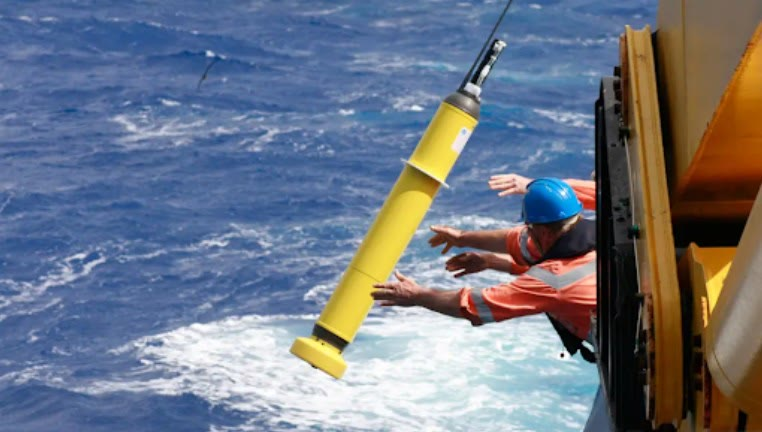
\includegraphics[width=\linewidth]{images/book5/b3-argo-deploy.jpg}

{\scriptsize Flotador Argo lanzado por la borda de un buque oceanográfico (NOAA
Global Ocean Monitoring and Observing Program, dominio público).}
\end{minipage}
\end{inthefield}
% ledger: argo:fleet, noaa:argo-25, photo:b3-argo-deploy

\section{Mareas oceánicas}\label{sec:b3:ocean-dynamics:tides}

Dos veces al día, con un retraso de algo menos de una hora cada día, el mar sube y
baja. Los libros de física explican la fuerza de marea: la atracción de la Luna es
más intensa en el lado de la Tierra más próximo a ella que en su centro, y más débil en el lado opuesto, de modo que, respecto al centro,
el agua se estira hacia fuera a lo largo de la
línea hacia la Luna a ambos lados.

\begin{definition}[Marea de equilibrio; componente de marea]\label{def:b3:ocean-dynamics:tides}
La \emph{marea de equilibrio}\index{marea de equilibrio} es la forma que
tomaría la superficie de un océano que cubriera toda la Tierra si siguiera
instantáneamente el potencial generador de marea, sin inercia. Una \emph{componente
de marea}\index{componente de marea} es uno de los términos armónicos, cada uno
con una frecuencia fija determinada por los movimientos de la Luna y el Sol, y una
amplitud y fase que se hallan en cada lugar, cuya suma constituye la marea; se
designan con una letra y el número de ciclos por día, como M$_2$, la
componente lunar semidiurna principal.
\end{definition}

\begin{theorem}[Marea de equilibrio de la Luna]\label{thm:b3:ocean-dynamics:equilibrium-tide}
Para la Luna, de masa $M$ a distancia $d$ del centro de la Tierra, de
masa $M_E$ y radio $a$, la \omterm{def:b3:ocean-dynamics:tides}{marea de equilibrio} en un ángulo $\theta$ desde
el punto bajo la Luna es
\[
\eta = K\,\frac{3\cos^2\theta - 1}{2},\qquad
K = \frac{M}{M_E}\Big(\frac{a}{d}\Big)^3 a .
\]
\end{theorem}

\begin{proof}
El potencial de la Luna en un punto a distancia $a$ del centro de la Tierra
y ángulo $\theta$ es $-GM/s$, con $s^2 = d^2 - 2ad\cos\theta +
a^2$. Desarrollando en $a/d$, $1/s = (1/d)[1 + (a/d)\cos\theta + (a/d)^2
(3\cos^2\theta - 1)/2 + \cdots]$. El primer término es una constante; el segundo
es un campo uniforme, el que acelera a toda la Tierra en su órbita
alrededor del centro de masas común, y no tiene efecto respecto a la Tierra.
Lo que queda es el potencial generador de marea $\Phi_T = -(GMa^2/d^3)(3
\cos^2\theta - 1)/2$. En equilibrio la superficie del mar es una superficie de
potencial total constante, $g\eta + \Phi_T = C$, con $g = GM_E/a^2$, así
$\eta = (M/M_E)(a^4/d^3)(3\cos^2\theta - 1)/2 + C/g$. La media de
$3\cos^2\theta - 1$ sobre la esfera vale cero; siendo el volumen de agua
constante, $C = 0$.
\end{proof}

Con el cociente de masas $0.0123$, $d = \qty{384400}{km}$ y $a =
\qty{6371}{km}$, $K = \qty{0.357}{m}$: el mar se eleva \qty{0.36}{m}
alta bajo la Luna y en el lado opuesto, y \qty{0.18}{m} por debajo en el
círculo máximo intermedio, un rango total de \qty{0.54}{m}. A la latitud $\varphi$, con
la Luna en declinación $\delta$ y ángulo horario $H$, $\cos\theta =
\sin\varphi\sin\delta + \cos\varphi\cos\delta\cos H$. Al girar la Tierra
bajo los dos abultamientos, un lugar pasa por dos pleamares en un día lunar,
\qty{24}{h} \qty{50}{min}: la marea semidiurna. Cuando la Luna se sitúa
al norte o al sur del ecuador los dos abultamientos quedan inclinados, y las dos pleamares
de un día son desiguales, como muestra la figura inferior. El Sol produce una
marea de la misma forma, con \num{0.46} veces su amplitud; ambas se suman en luna nueva y
llena, en las mareas vivas, y se compensan en parte en los cuartos.
% ledger: moon5:orbit, earth:Rmean, stewart:tide-equilibrium (computed in figdata/bachelor-3/tides.py)

\begin{omfigure}
\begin{tikzpicture}
\begin{groupplot}[group style={group size=2 by 1, horizontal sep=1.9cm},
  tick label style={font=\scriptsize}, label style={font=\small},
  legend style={font=\scriptsize, draw=none, fill=none}]
\nextgroupplot[width=0.40\linewidth, height=0.40\linewidth, axis equal image, hide axis,
  clip=false, xmin=-1.3, xmax=2.0, ymin=-1.25, ymax=1.25]
% computed in figdata/bachelor-3/tides.py
\addplot[fill=omThm!12, draw=omThm, thick] table[x=x, y=y] {figdata/out/bachelor-3-tides-bulge.dat};
\addplot[black, fill=black!10, domain=0:360, samples=91] ({cos(x)}, {sin(x)});
\draw[->, >=stealth, thick] (axis cs:1.25,0) -- (axis cs:1.95,0);
\node[above, font=\scriptsize, align=center] at (axis cs:1.6,0.08) {hacia la\\Luna};
\node[font=\scriptsize] at (axis cs:0,0) {Tierra};
\nextgroupplot[width=0.54\linewidth, height=0.40\linewidth, xlabel={tiempo (\unit{h})},
  ylabel={$\eta$ (\unit{m})}, xmin=0, xmax=49.6, xtick={0,12,24,36,48}, ymin=-0.2, ymax=0.4,
  legend style={at={(axis cs:12.4,0.39)}, anchor=north}, legend cell align=left, legend columns=2]
\addplot[omDef, thick] table[x=t, y=eta0] {figdata/out/bachelor-3-tides-series.dat};
\addlegendentry{$\delta = 0$}
\addplot[omThm, thick] table[x=t, y=eta20] {figdata/out/bachelor-3-tides-series.dat};
\addlegendentry{$\delta = \ang{20}$}
\addplot[black!50, thin, forget plot] coordinates {(0,0) (49.6,0)};
\end{groupplot}
\end{tikzpicture}

\par\smallskip{\small A la izquierda, la \omterm{def:b3:ocean-dynamics:tides}{marea de equilibrio} de la Luna, en el plano
que contiene a la Luna, con el abultamiento exagerado unas dos millones de veces.
A la derecha, la \omterm{def:b3:ocean-dynamics:tides}{marea de equilibrio} a \ang{45} N durante dos días lunares, con la
Luna en el ecuador (azul) y en declinación \ang{20} N (rojo): el segundo
caso tiene una pleamar mucho más alta que la otra, la
desigualdad diurna.}\label{fig:b3:ocean-dynamics:equilibrium-tide}
\end{omfigure}
% ledger: moon5:orbit, stewart:tide-constituents

El análisis armónico de la \omterm{def:b3:ocean-dynamics:tides}{marea de equilibrio} proporciona sus componentes. Las
cinco mayores, con sus amplitudes de equilibrio, figuran en la tabla inferior. Al
menos 39 componentes son necesarias para predecir la marea de un puerto con una
precisión de una milésima de su término mayor, y un mareógrafo debe registrar más de 18.6 años, el
periodo de la modulación de las mareas lunares, para separarlas todas.

\begin{center}
\small
\begin{tabular}{llrr}
\hline
componente & origen & periodo (\unit{h}) & amplitud de equilibrio (\unit{m}) \\
\hline
M$_2$ & lunar principal, semidiurna & \num{12.4206} & \num{0.2423} \\
S$_2$ & solar principal, semidiurna & \num{12.0000} & \num{0.1128} \\
N$_2$ & lunar elíptica, semidiurna & \num{12.6584} & \num{0.0464} \\
K$_1$ & lunisolar, diurna & \num{23.9344} & \num{0.1416} \\
O$_1$ & lunar principal, diurna & \num{25.8194} & \num{0.1005} \\
\hline
\end{tabular}
\end{center}
% ledger: stewart:tide-constituents, stewart:tide-prediction

La marea real no es la \omterm{def:b3:ocean-dynamics:tides}{marea de equilibrio}. Para mantener un abultamiento bajo la Luna
en el ecuador, la marea tendría que recorrer la Tierra en un día lunar,
a unos \qty{460}{m/s}, una velocidad que una onda de gravedad larga solo alcanza
en un océano de \qty{22}{km} de profundidad; y los continentes la detienen. La marea es
en realidad una onda larga forzada, que oscila en cada cuenca cerca de la resonancia, y la
rotación de la Tierra hace que gire alrededor de la cuenca.
% ledger: stewart:tide-prediction

\begin{definition}[Onda de Kelvin]\label{def:b3:ocean-dynamics:kelvin-wave}
Una \emph{onda de Kelvin}\index{onda de Kelvin} oceánica es una onda de gravedad larga
que se propaga a lo largo de una costa, o a lo largo del ecuador, sin velocidad transversal
a ella, con su altura disminuyendo exponencialmente al alejarse de la costa sobre el
radio de Rossby. A lo largo de una costa se propaga con la costa a su derecha en el
hemisferio norte, a su izquierda en el sur.
\end{definition}

\begin{theorem}[Onda de Kelvin costera]\label{thm:b3:ocean-dynamics:kelvin}
En un océano de profundidad uniforme $H$ sobre un plano $f$, con $f > 0$, limitado por una
costa recta a lo largo de $y = 0$ y situado en $y > 0$, las ecuaciones lineales de aguas someras
tienen las soluciones con $v = 0$
\[
\eta = \mathrm e^{-y/L_R}F(x - ct),\qquad u = \frac{g}{c}\,\eta,\qquad
c = \sqrt{gH},\quad L_R = \frac{c}{f},
\]
para cualquier perfil $F$, y ninguna solución con $v = 0$ se propaga en la dirección
$-x$.
\end{theorem}

\begin{proof}
Con $v = 0$ las ecuaciones son $\partial u/\partial t = -g\,\partial\eta/
\partial x$, $fu = -g\,\partial\eta/\partial y$ y $\partial\eta/\partial t
+ H\,\partial u/\partial x = 0$. La primera y la tercera dan $\partial^2
\eta/\partial t^2 = gH\,\partial^2\eta/\partial x^2$: en $x$ cada línea
$y = $ constante transporta ondas $F(x \mp ct)$ con $c = \sqrt{gH}$, y luego la
primera ecuación da $u = \pm(g/c)\eta$. La segunda se convierte en $\partial\eta/
\partial y = \mp(f/c)\eta$, así que $\eta \propto \mathrm e^{\mp y/L_R}$. Con
el signo superior, la onda decae alejándose de la costa; con el inferior
crecería sin límite hacia el océano, lo que queda excluido. La onda avanza
hacia $+x$ con el océano a su izquierda y la costa a su derecha.
\end{proof}

En el océano profundo, de \qty{4000}{m} de profundidad, $c = \qty{198}{m/s}$ y el
radio de Rossby es de unos \qty{2000}{km} en latitudes medias: la marea recorre
toda una cuenca. Sobre un mar de plataforma de \qty{50}{m} de profundidad, $c =
\qty{22}{m/s}$, el radio de Rossby es inferior a \qty{200}{km}, y una longitud de onda de M$_2$
es de unos \qty{1000}{km}. En un golfo, la marea que entra a lo largo de una
costa como \omterm{def:b3:ocean-dynamics:kelvin-wave}{onda de Kelvin} regresa por la costa opuesta, de nuevo con la
costa a su derecha; las dos ondas se anulan en puntos intermedios.

\begin{definition}[Punto anfidrómico; línea cotidal; línea de igual amplitud]\label{def:b3:ocean-dynamics:amphidrome}
Un \emph{punto anfidrómico}\index{punto anfidrómico} es un punto en el que la
amplitud de una \omterm{def:b3:ocean-dynamics:tides}{componente de marea} es nula y alrededor del cual
gira la pleamar. Una \emph{línea cotidal}\index{línea cotidal} une los lugares donde
la pleamar de una componente llega a la misma hora; una \emph{línea de
igual amplitud}\index{línea de igual amplitud} une los lugares de igual rango de marea. Las
líneas cotidales irradian desde los puntos anfidrómicos; las líneas de igual amplitud los rodean.
\end{definition}

\begin{omfigure}
\centering
\begin{tikzpicture}
\begin{axis}[width=0.96\linewidth, height=0.35\linewidth, axis equal image,
  xmin=0, xmax=1600, ymin=0, ymax=400, xtick={0,400,800,1200,1600}, ytick={0,200,400},
  xlabel={distancia a lo largo del canal (\unit{km})}, ylabel={a través del canal (\unit{km})},
  tick label style={font=\scriptsize}, label style={font=\small}]
% computed in figdata/bachelor-3/tides.py
\addplot[omDef!70, densely dashed, unbounded coords=jump] table[x=x, y=y] {figdata/out/bachelor-3-tides-cor.dat};
\pgfplotsinvokeforeach{30,60,90,120,150,180,210,240,270,300,330}{
  \addplot[omThm, thin, unbounded coords=jump] table[x=x, y=y] {figdata/out/bachelor-3-tides-cot-#1.dat};
}
\addplot[omThm, very thick, unbounded coords=jump] table[x=x, y=y] {figdata/out/bachelor-3-tides-cot-0.dat};
\addplot[only marks, mark=*, mark size=2pt] table[x=x, y=y] {figdata/out/bachelor-3-tides-amph.dat};
\addplot[->, >=stealth, very thick, domain=20:310, samples=60] ({742.7+70*cos(x)}, {200+70*sin(x)});
\end{axis}
\end{tikzpicture}

\par\smallskip{\small Dos \omterm{def:b3:ocean-dynamics:kelvin-wave}{ondas de Kelvin} de la marea M$_2$ en un
canal ficticio de \qty{400}{km} de anchura y \qty{50}{m} de profundidad a \ang{55} N, una de ellas hacia
el este por la costa sur, la otra hacia el oeste por la costa norte.
En rojo, las \omterm{def:b3:ocean-dynamics:amphidrome}{líneas cotidales}, cada \ang{30} de fase (aproximadamente una hora), la
más gruesa para la pleamar en el instante origen; en azul discontinuo, las \omterm{def:b3:ocean-dynamics:amphidrome}{líneas de
igual amplitud}, cada quinta parte de la amplitud de una onda en su costa. Los
\omterm{def:b3:ocean-dynamics:amphidrome}{puntos anfidrómicos} (marcados con puntos) están sobre la línea central a media longitud de onda,
\qty{495}{km} de distancia entre sí, y la pleamar gira alrededor de ellos en sentido antihorario
(flecha).}\label{fig:b3:ocean-dynamics:amphidromes}
\end{omfigure}

Los mapas de la marea oceánica obtenidos por satélite, con una precisión de unos
\qty{2}{cm} en mar profundo, muestran esta estructura en todas partes: la M$_2$
cresta gira en sentido antihorario alrededor de los \omterm{def:b3:ocean-dynamics:amphidrome}{puntos anfidrómicos} de las cuencas
del hemisferio norte y en sentido horario en el hemisferio sur, y los mayores rangos se dan en las
costas. Las mareas disipan \qty{3.75}{TW}, de los cuales \qty{3.5}{TW} en el
océano, unas dos terceras partes de la energía de M$_2$ en las plataformas y en mares someros
y un tercio mediante ondas internas en el océano profundo. Esa energía
alarga el día unos \qty{2.07}{ms} por siglo y aleja la Luna
\qty{3.86}{cm} al año; y la parte disipada en el océano profundo mezcla las aguas,
aportando parte de la mezcla que, en el esquema de Stommel--Arons, impulsa
la circulación abisal.
% ledger: stewart:tide-prediction


\section{Ejercicios}

\begin{exercise}[$\star$]\label{exo:b3:ocean-dynamics:1}
Una tensión del viento del oeste de \qty{0.12}{Pa} sopla sobre el mar a \ang{40} N
($\rho = \qty{1025}{kg/m^3}$, $\Omega = \qty{7.292115e-5}{rad/s}$).
Calcúlese el transporte de volumen de Ekman por metro de anchura y su dirección,
y el transporte a través de una sección de \qty{1000}{km} de longitud, en sverdrups.
\end{exercise}

\begin{exercise}[$\star$]\label{exo:b3:ocean-dynamics:2}
Con $A_z = \qty{0.05}{m^2/s}$, calcúlese la \omterm{def:b3:ocean-dynamics:ekman-pumping}{profundidad de Ekman} a \ang{45} N. ¿Qué
fracción de la corriente superficial queda a esa profundidad?
\end{exercise}

\begin{exercise}[$\star$]\label{exo:b3:ocean-dynamics:3}
A \ang{30} N el rotacional de la tensión del viento es \qty{-1e-7}{Pa/m} a lo ancho de una
cuenca de \qty{5000}{km} de anchura ($a = \qty{6371}{km}$). Calcúlese $\beta$, el
transporte de Sverdrup por unidad de anchura y el transporte total, con su
dirección.
\end{exercise}

\begin{exercise}[$\star$]\label{exo:b3:ocean-dynamics:4}
A partir de los periodos de M$_2$ y S$_2$, calcúlese el periodo del ciclo de
mareas vivas y muertas, el tiempo que transcurre entre dos alineaciones de
ambas \omterm{def:b3:ocean-dynamics:tides}{componentes de marea}.
\end{exercise}

\begin{exercise}[$\star\star$]\label{exo:b3:ocean-dynamics:5}
Un esfuerzo del viento del oeste crece linealmente desde 0 en \ang{35} N hasta \qty{0.1}{Pa} en
\ang{45} N, \qty{1110}{km} más al norte. Calcúlese el \omterm{def:b3:ocean-dynamics:ekman-pumping}{bombeo de Ekman} en
\ang{40} N, conservando ambos términos de la \cref{prop:b3:ocean-dynamics:pumping}, en
metros por año. ¿Se empuja el agua hacia arriba o hacia abajo?
\end{exercise}

\begin{exercise}[$\star\star$]\label{exo:b3:ocean-dynamics:6}
En un giro de Stommel con $r = \qty{2e-6}{s^{-1}}$ y $\beta =
\qty{2e-11}{m^{-1}.s^{-1}}$, calcúlese la anchura $\delta_S$. Si la corriente de
frontera transporta \qty{30}{\sverdrup} en los \qty{800}{m} superiores, dentro de una
anchura $\delta_S$, ¿cuál es su velocidad media?
\end{exercise}

\begin{exercise}[$\star\star$]\label{exo:b3:ocean-dynamics:7}
Calcúlense la anchura de Munk $\delta_M$ y la anchura del chorro hacia el norte,
$(2\pi/\sqrt3)\,\delta_M$, a \ang{30} N para $A_H = \qty{e4}{m^2/s}$. ¿Cómo
varía la anchura si $A_H$ es ocho veces menor?
\end{exercise}

\begin{exercise}[$\star\star$]\label{exo:b3:ocean-dynamics:8}
Dos estaciones separadas \qty{80}{km} se sitúan sobre una línea que va del oeste ($A$) al este
($B$) a \ang{36} N. Respecto a la superficie de \qty{1000}{dbar}, la
anomalía \omterm{def:b3:gravity-geodesy:geopotential}{geopotencial} de la superficie del mar es \qty{14.5}{J/kg} en $A$ y
\qty{21.3}{J/kg} en $B$. Calcúlese la corriente superficial respecto a
\qty{1000}{dbar} y su dirección. ¿Qué estación tiene la columna de agua
más cálida?
\end{exercise}

\begin{exercise}[$\star\star$]\label{exo:b3:ocean-dynamics:9}
Con la \omterm{def:b3:ocean-dynamics:tides}{marea de equilibrio} de la Luna, $K = \qty{0.357}{m}$, y la razón
\num{0.46} de la marea solar a la lunar, calcúlese el rango mareal de equilibrio
(pleamar bajo los astros menos bajamar a \ang{90}) en mareas vivas y en
mareas muertas, y su razón.
\end{exercise}

\begin{exercise}[$\star\star\star$]\label{exo:b3:ocean-dynamics:10}
En el plano $\beta$ ecuatorial, $f = \beta_0y$ con $\beta_0 =
2\Omega/a$. Demuéstrese que la \omterm{def:b3:ocean-dynamics:kelvin-wave}{onda de Kelvin} $\eta = G(y)F(x - ct)$, $v = 0$,
se convierte en $G = \exp(-\beta_0y^2/2c)$, atrapada a ambos lados del ecuador,
y se propaga hacia el este. Calcúlese su escala de atrapamiento $\sqrt{c/\beta_0}$ para una
onda de velocidad \qty{2.5}{m/s}.
\end{exercise}

\begin{exercise}[$\star\star\star$]\label{exo:b3:ocean-dynamics:11}
(a)~Deríbese $V = a\tan\varphi\,W_0$ para el interior abisal a partir de $\beta v =
f\,\partial w/\partial z$. (b)~Con $W_0 = \qty{e-7}{m/s}$, calcúlese $V$ a
\ang{30} N y el transporte total hacia el polo a través de una cuenca
de \qty{5000}{km} de anchura. (c)~¿De dónde debe proceder el agua?
\end{exercise}

\begin{exercise}[$\star\star\star$]\label{exo:b3:ocean-dynamics:12}
Una corriente geostrófica $W_g = u_g + \mathrm iv_g$ fluye sobre un fondo marino
plano en $z = 0$, con viscosidad de remolino $A_z$ y sin deslizamiento en el fondo.
(a)~Demuéstrese que $W = W_g(1 - \mathrm e^{-(1+\mathrm i)z/\delta})$, $\delta =
\sqrt{2A_z/f}$. (b)~Demuéstrese que el defecto de transporte de esta capa de Ekman de fondo
bombea la velocidad vertical $w = \tfrac12\delta\zeta_g$ hacia el
interior, siendo $\zeta_g$ la vorticidad de la corriente geostrófica. (c)~Para
$A_z = \qty{0.01}{m^2/s}$, $f = \qty{e-4}{s^{-1}}$ y un océano
de \qty{4000}{m} de profundidad, calcúlese $\delta$, la tasa de frenado $r =
f\delta/2H$, y su inversa en días.
\end{exercise}
% ledger: earth:Rmean, geod5:grs80-defining, stewart:tide-constituents, stewart:tide-equilibrium

\section{Problema: un giro en el mar de Ammar}

\begin{problem}[{Problema de fin de semana --- bombeo de Ekman, transporte de Sverdrup,
la corriente de frontera occidental y la marea de un océano inventado}]
\label{pb:b3:ocean-dynamics:1}
El mar de Ammar es una cuenca oceánica inventada, un rectángulo desde \ang{20} hasta
\ang{50} N y de \qty{6000}{km} de anchura y \qty{4000}{m} de profundidad. La tensión del viento es
zonal, $\tau_x = -\tau_0\cos(\pi(\varphi - \ang{20})/\ang{30})$ con $\tau_0
= \qty{0.1}{Pa}$. Se toman $\rho = \qty{1025}{kg/m^3}$, $\Omega =
\qty{7.292115e-5}{rad/s}$, $a = \qty{6371}{km}$, $g = \qty{9.81}{m/s^2}$,
y, cuando se pida un plano $\beta$, su valor a \ang{35} N.

\medskip\noindent\textbf{Parte I --- La capa de Ekman.}
\begin{enumerate}
\item Calcúlese la tensión del viento a \ang{20}, \ang{35} y \ang{50} N.
\item Calcúlese $f$ a las mismas latitudes.
\item Calcúlese el transporte de volumen de Ekman por unidad de anchura a \ang{20} y
  \ang{50} N, con su dirección. ¿Convergen o divergen los transportes en
  la cuenca?
\item Con $A_z = \qty{0.05}{m^2/s}$, calcúlese la \omterm{def:b3:ocean-dynamics:ekman-pumping}{profundidad de Ekman} a \ang{35} N.
\item Calcúlese el \omterm{def:b3:ocean-dynamics:ekman-pumping}{bombeo de Ekman} a \ang{35} N, en metros por segundo y por
  año.
\item ¿Cuántos años tardaría este bombeo en hacer descender el agua superficial
  \qty{500}{m}?
\end{enumerate}

\medskip\noindent\textbf{Parte II --- El interior de Sverdrup.}
\begin{enumerate}[resume]
\item Calcúlese la longitud $L$ de la cuenca de sur a norte y $\beta$ a
  \ang{35} N.
\item Calcúlese el rotacional de la tensión del viento a \ang{35} N.
\item Calcúlese el transporte de Sverdrup por unidad de anchura a \ang{35} N, con su
  dirección.
\item Calcúlese el transporte total del interior a través de la cuenca a \ang{35} N,
  en sverdrups.
\item Si este flujo se reparte en los \qty{1000}{m} superiores, ¿cuál es su
  velocidad media, y cuántos años tarda una porción de agua en desplazarse \qty{1000}{km}
  hacia el sur?
\item Demuéstrese que $fw_E/\beta$ a \ang{35} N da el mismo transporte, y
  explíquese por qué, con la \omterm{def:b3:atmospheric-dynamics:pv}{vorticidad potencial} de una columna.
\end{enumerate}

\medskip\noindent\textbf{Parte III --- La corriente de frontera occidental.}
\begin{enumerate}[resume]
\item Explíquese por qué el flujo de retorno no puede discurrir por el lado oriental de la
  cuenca.
\item Con una fricción de fondo $r = \qty{e-6}{s^{-1}}$, calcúlese la
  anchura de Stommel $\delta_S$.
\item Calcúlese el transporte hacia el norte por unidad de anchura en la pared occidental,
  $A(X/\delta_S - 1)$, y la velocidad media si ocupa los
  \qty{1000}{m} superiores.
\item ¿A qué distancia de la pared termina el flujo hacia el norte?
\item Calcúlese el transporte hacia el norte de la capa límite de Stommel, y
  explíquese por qué queda por debajo del transporte del interior en unos
  \qty{1.5}{\sverdrup}.
\item Con $A_H = \qty{5e3}{m^2/s}$, calcúlese $\delta_M$ y la anchura del
  chorro de Munk hacia el norte.
\item El chorro de Munk transporta $1 + \mathrm e^{-\pi/\sqrt3}$ veces el transporte del
  interior. Calcúlese, y dígase a dónde va el exceso.
\end{enumerate}

\medskip\noindent\textbf{Parte IV --- La marea del mar de Ammar.}
\begin{enumerate}[resume]
\item Calcúlese la velocidad de una \omterm{def:b3:ocean-dynamics:kelvin-wave}{onda de Kelvin} en la cuenca y el radio de Rossby
  a \ang{35} N.
\item Calcúlese la longitud de onda de la \omterm{def:b3:ocean-dynamics:kelvin-wave}{onda de Kelvin} de M$_2$.
\item ¿Cuánto tarda una \omterm{def:b3:ocean-dynamics:kelvin-wave}{onda de Kelvin} en recorrer una vez las costas de
  la cuenca, y cuántos periodos de M$_2$ son?
\item ¿A qué velocidad tendría que desplazarse la \omterm{def:b3:ocean-dynamics:tides}{marea de equilibrio} alrededor del
  círculo de \ang{35} N para mantenerse bajo la Luna, y en qué profundidad de océano
  se propagaría tan rápido una onda larga?
\item ¿Dónde cabría esperar el \omterm{def:b3:ocean-dynamics:amphidrome}{punto anfidrómico} de la cuenca, y en qué
  sentido gira la pleamar alrededor de él?
\item Calcúlese la amplitud de equilibrio semidiurna a \ang{35} N, $\tfrac34
  K\cos^2\varphi$, con $K = \qty{0.357}{m}$, para la Luna situada sobre el ecuador.
\item Indíquese el transporte de la corriente de frontera occidental que cierra el
  giro del mar de Ammar.
\end{enumerate}
\end{problem}
% ledger: earth:Rmean, geod5:grs80-defining, stewart:tide-constituents
